%%%%%%%%%%%%%%%%%%%%%%%%%%%%%%%%%%%%%
\section{Methods}
\label{sec:Methods}

\subsection{GEANT4 Implemenation}

A large focus of this work was on creating a working simulation of the GEANT4 toolkit.
Prelimary attemps were made to install GEANT4 on a windows based machine linking to Microscoft Visual Studio. While these attempts were sucessful, a larger scale computing enviroment was desired.
GEANT4 was then installed on the University of Tennessee's nuclear engineering computing cluster, along with the necessary visualation drivers and data files.
Brief documenation on compiling simple examples on the cluster are aviable at \url{necluster.engr.utk.edu/wiki/index.php/Geant4}\footnote{It should be noted that this example uses the CMAKE build system (as per the GEANT4 recommendation) but a large majority of the examples still use GNUMake for building. This can be accomplished by adding \verb+source /opt/geant4/geant4-9.5p1/share/Geant4-9.5.1/geant4make/geant4make.sh+ to the user's \verb+.bashrc+.}. 
For convince a subversion repository was created to manage the developed code base, and all source code is available by anonymous checkout from \url{http://www.murphs-code-repository.googlecode.com/svn/trunk/layeredPolymerTracking}. Revision 360 was the code base used to generate the results shown in \ref{sec:Results}.
The following section provides implemenation specific details of the code base used to simulate the energy deposition in thin films.
It is organzied according to the three base classes that a user must implement in GEANT4, namely \verb+G4VUserDetectorConstruciton+, \verb+G4VUserPhysicsList+, and \verb+G4VuserPrimaryGeneratorAction+.
\subsubsection{Detector Geometry}
A detector geometry in GEANT4 is made up of a number of volumes.
The largest volume is the \verb+world+ volume which contains all other volumes in the detector geometry.
Each volume (an instance of \verb+G4VPhysicalVolume+) by assigning a position, a pointer to the mother volume and a pointer to its mother volume (or \verb+NULL+ if it is the \verb+world+ volume).
A volume's shape is described by \verb+G4VSolid+ which has a shape and the specific values for each dimension.
A volume's full properties is described by a logical volume.
A \verb+G4LogicalVolume+ includes a pointer to the geometrical properties of the volume (the solid) along with physical characteristics including:
\begin{itemize}
    \item the material of the volume,
    \item sensitive detectors of the volume and,
    \item any magnetic fields.
\end{itemize}
Listing \ref{lst:World} provides the implementation of the world physical volume.
The geometry was setup such that it is possible to define multiple layers of detectors, as shown in Figure \ref{fig:LayerDetectorGeo}.
%%%%%%%%%%%%%%%%%%%%%%%%% LISTING CODE %%%%%%%%%%%%%%%%%%%%%%%%%%
\lstinputlisting[linerange={217-220},caption=World Physical Volume,label=lst:World]{src/DetectorConstruction.cc}
The detector was described by creating creating a single layer of neutron absorber and gap material and placing it in another volume (the calorimeter).
The containing volume (calorimeter) was placed inside of the the physical world (Listing \ref{lst:Calo}).
%%%%%%%%%%%%%%%%%%%%%%%%% LISTING CODE %%%%%%%%%%%%%%%%%%%%%%%%%%
\lstinputlisting[linerange={226-229},caption=Calorimeter Volume,label=lst:Calo]{src/DetectorConstruction.cc}
The \verb+calorimeter+ was the mother volume for each layer. 
The code was developed such that the simulation of multiple layers can be easily set at compile time or by utilizing a run macro through the \verb+DetectorMessenger+ class.
Multiple repeated volume can be achieved in GEANT4 through \verb+G4PVReplica+ or \verb+G4PVParameterised+.
As each of the layers had the same geometry, \verb+G4PVReplica+ was chosen as the implementation (Listing \ref{lst:Layer}.
%%%%%%%%%%%%%%%%%%%%%%%%% LISTING CODE %%%%%%%%%%%%%%%%%%%%%%%%%%
\lstinputlisting[linerange={231-238},caption=Layer Volume,label=lst:Layer]{src/DetectorConstruction.cc}
Finally, the neutron absorber and gap material were defined as single cylinders which were then placed in the layer mother volume (Listing \ref{lst:GapAbs}).
The size of these solids (and the materials) could be set either at compile time through \verb+DetectorConstruction+ constructor or by using the \verb+DetectorMessenger+ in the run macro.
%%%%%%%%%%%%%%%%%%%%%%%%% LISTING CODE %%%%%%%%%%%%%%%%%%%%%%%%%%
\lstinputlisting[linerange={241-249},caption=Absorber and Gap Volumes,label=lst:GapAbs]{src/DetectorConstruction.cc}
Figure \ref{fig:LayerDetectorGeo} shows a rendering of the 10 layers of the detector with the trajectories from a gamma event.
\begin{figure} 
    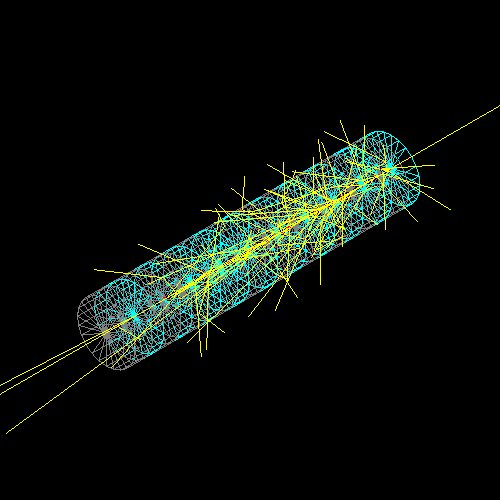
\includegraphics[width=\figurewidth]{10LayerGamma}
	\caption{10 Layer Detector with a simulated gamma event}
    \label{fig:LayerDetectorGeo}
\end{figure}

\subsubsection{Physics Lists}
The user of the GEANT4 toolkit is responsible for selecting the proper physics processes to model in the \verb+PhysicsList+.
This is unlike other transport codes (such as MCNPX) where basic physics are enabled by default and the user only has select the appropriate cards.
However, GEANT4 does provide examples of implemented \verb+PhysicsLists+ as wells as modular physics lists which provide a way to construct a physics list by combing physics list.
Thus, extensive use of \verb+G4ModularPhysicsList+ was employed to handle the assigning of the physics processes to each particle in the correct order.
The physics lists chosen for this simulation are listed below:
\begin{itemize}
    \item \verb+G4EmStandardPhysics+
    \item \verb+G4EmLivermorePhysics+
    \item \verb+HadronPhysicsQGSP_BERT_HP+ Hadronic physics are
    \item \verb+G4IonPhysics+ Finally, to handle the transport of the charged ions resulting from an ${}^6\text{Li}(\text(n),\alpha){}^{3}\text{H}$ interaction the \verb+G4IonPhysics+ list was used.
\end{itemize}
%%%%%%%%%%%%%%%%%%%%%%%%% LISTING CODE %%%%%%%%%%%%%%%%%%%%%%%%%%
\lstinputlisting[linerange={10-25},caption=Implemented Physics List,label=lst:PhysicsListCtr]{src/PhysicsList.cc}
Finally, the default cut range was decreased from 1 cm to 1 nm in \verb+SetCuts()+ (Listing \ref{lst:PhyisicsListSetCuts}) 
%%%%%%%%%%%%%%%%%%%%%%%%% LISTING CODE %%%%%%%%%%%%%%%%%%%%%%%%%%
\lstinputlisting[linerange={38-40},caption=Implemented Physics List,label=lst:PhysicsListSetCuts]{src/PhysicsList.cc}


\subsection{Determination of Single Collision Energy Loss Spectra}

\subsection{Determination of Energy Deposition}
